\begin{definition}{Markovian Decision Processes}{mdp}
    Un \textbf{Markovian Decision Process} (MDP) est un modèle de processus de décision séquentiel dans lequel les états sont Markoviens. Un MDP est défini par un tuple $\langle S, A, T, R, \gamma \rangle$ où:
    \begin{itemize}
        \item $S$ est un ensemble fini d'états;
        \item $A$ est un ensemble fini d'actions;
        \item $T : S \times A \times S \rightarrow [0, 1]$ est la fonction de transition. On a que $T(s, a, s') = P(s' | s, a)$ qui est la probabilité de passer de l'état $s$ à l'état $s'$ en effectuant l'action $a$;
        \item $R : S \times A \times S \rightarrow \mathbb{R}$ est la fonction de récompense;
        \item $S_0$ est l'état initial;
        \item $S_T$ est l'état terminal;
        % \item $\gamma \in [0, 1]$ est le facteur d'actualisation. 
    \end{itemize}
\end{definition}

Nous sommes donc dans un environnement \textbf{Non-Déterministe}, 
\textbf{Séquentiel}, \textbf{Statique}, \textbf{Discret} et \textbf{Complètement observable}. 
Une action $a$ n'a pas toujours le même effet dans un état $s$ donné. En effet, 
il y a une probabilité $T(s, a, s')$ que l'action $a$ dans l'état $s$ nous amène à l'état $s'$. 

Dans une recherche déterministe, nous pouvons toujours déterminer l'état suivant. Par ce fait 
nous voulions établir un \textbf{plan} qui est une séquence d'actions qui nous amène à l'état final. 
Dans un MDP, nous ne pouvons pas établir un plan car nous ne pouvons pas déterminer l'état suivant à 100\%
de certitude. Nous devons donc établir une \textbf{politique} qui est une fonction qui nous dit quelle action 
prendre dans un état donné. 

\begin{definition}{Politique}{policy}
    Une \textbf{politique} est une fonction $\pi : S \rightarrow A$ qui nous dit quelle action prendre dans un état donné. 
    La politique \textbf{optimale} est la politique qui maximise l'utilité, notée $\pi^*$.
\end{definition}

\begin{remark}\leavevmode
    Un plan n'est pas une bonne idée dans un environnement non-déterministe car il peut y avoir des 
    changements dans l'environnement qui rendent le plan \textbf{obsolète}.
\end{remark}

\begin{example}\leavevmode
    Imaginons une voiture qui peut se déplacer soit rapidement, soit lentement. 
    En fonction de ses actions, elle est soite $Cool$, $Warm$ ou $Overheated$.
    Voici la représentation via un automate: 
    \begin{figure}[H]
        \centering
        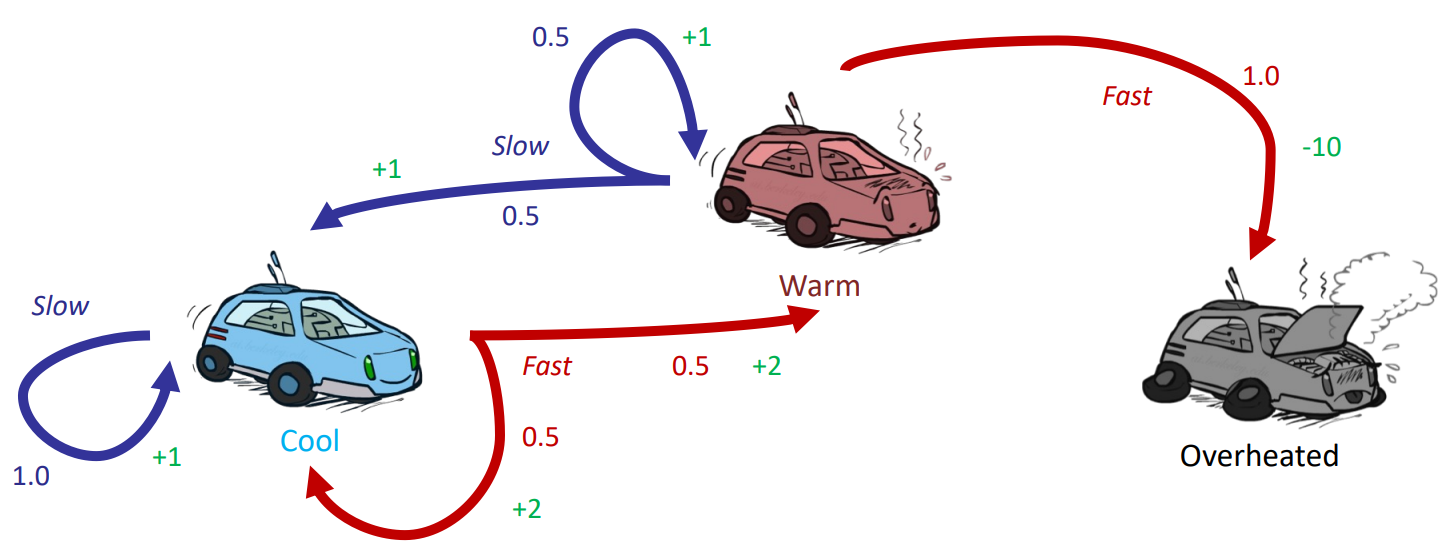
\includegraphics[width=0.4\textwidth]{pictures/automateracing.png}
        \hspace{2cm}
        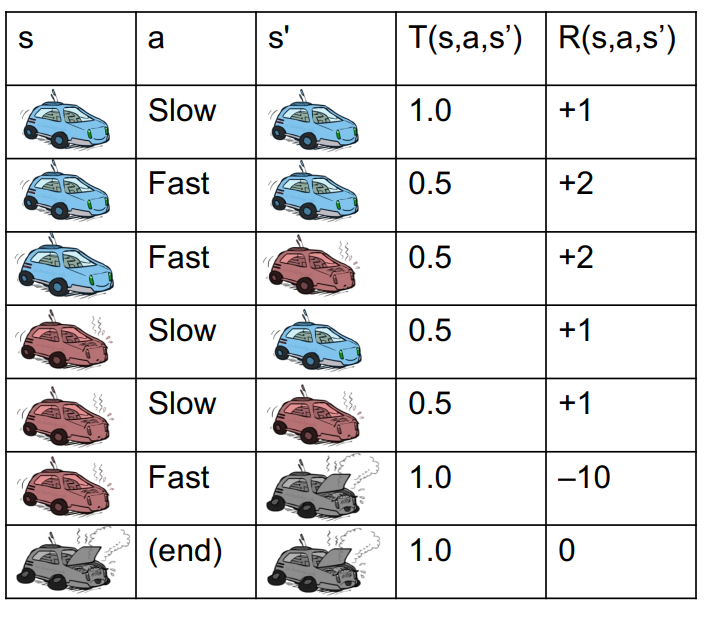
\includegraphics[width=0.4\textwidth]{pictures/tableracing.png}
        \caption{Voiture de course (kachow)}\label{fig:automateracing}
    \end{figure}

\end{example}

Nous pouvons alors représenter l'arbre de recherche de la voiture de course comme suit: 
\begin{figure}[H]
    \centering
    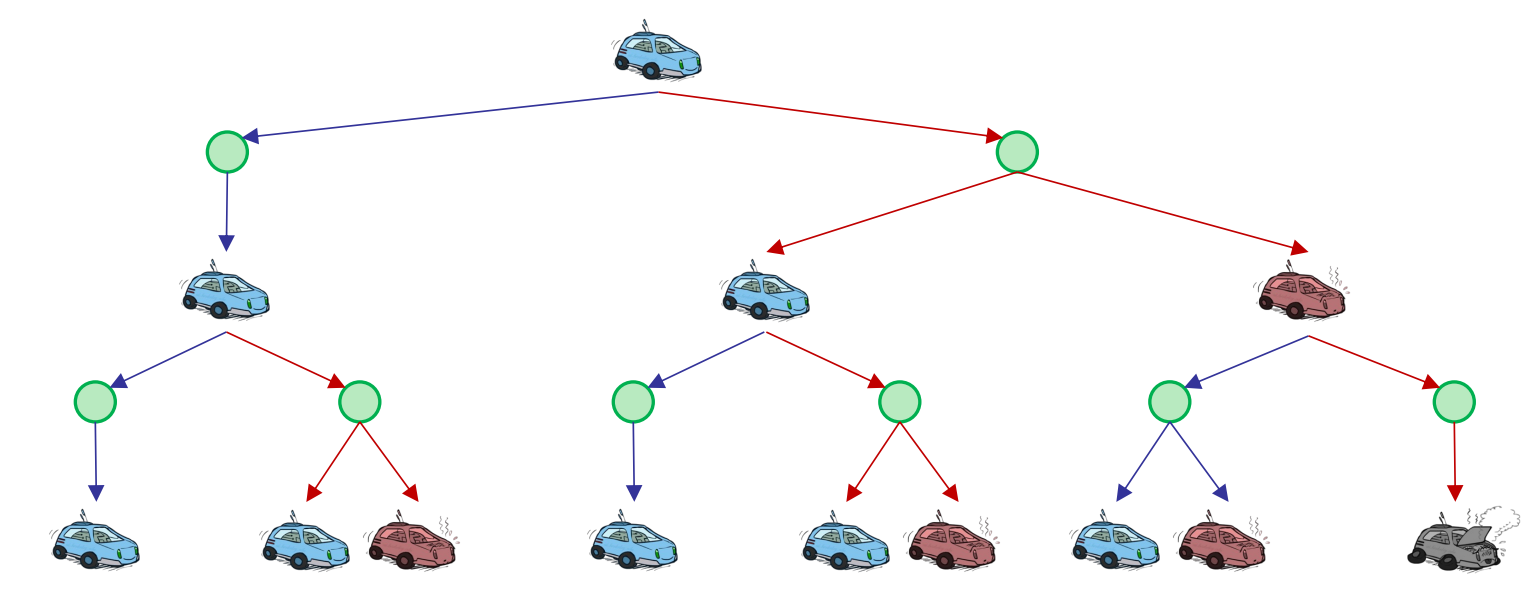
\includegraphics[width=0.95\textwidth]{pictures/racingtree.png}
    \caption{Arbre de recherche}\label{fig:racingtree}
\end{figure}
Nous pouvons faire un lien entre la représentation de l'arbre et l'arbre de l'algorithme \textbf{Expectimax} 
vu précédemment. En effet, nous pouvons voir que les \textcolor{green}{nœuds chance} sont les nœuds où la voiture peut 
changer d'état en fonction d'une action.

\subsection{Hyper-Paramètres} % (fold)
\label{sub:hyper_parametres}

\begin{definition}{Discount Factor}{gamma}
    Le \textbf{discount factor} $\gamma$ est un hyper-paramètre qui représente l'importance des récompenses futures. 
    Plus $\gamma$ est proche de 1 ou supérieur, plus les récompenses futures sont importantes.
    Plus $\gamma$ est proche de 0, plus les récompenses futures sont négligeables. 
    \begin{itemize}
        \item $\gamma = 0$: \textbf{Myopic} (court-termiste);
        \item $\gamma = 1+$: \textbf{Far-sighted} (long-termiste);
    \end{itemize}  
    Si $\gamma = 1$, les récompenses futures sont aussi importantes que les récompenses actuelles.

    A chaque étape de la recherche, nous multiplions la récompense par $\gamma^k$ où $k$ est le nombre d'étapes
\end{definition}

\begin{definition}{Living Reward}{}
    Le \textbf{living reward} est une récompense négative qui est donnée à chaque étape de la recherche. 
    Cela permet d'éviter que l'agent ne reste dans un état pendant trop longtemps.
\end{definition}

\begin{definition}{Noise}{}
    Le \textbf{noise} est un hyper-paramètre qui représente la probabilité que l'action choisie ne soit pas celle effectuée. 
    Cela permet de représenter le fait que l'agent ne peut pas toujours effectuer l'action qu'il veut. 
    Par exemple, si l'agent veut aller à gauche, il peut y avoir un obstacle qui l'en empêche et va donc aller à droite.
    Le noise permet de représenter ce genre de situation.
\end{definition}

\begin{figure}[H]
    \centering
    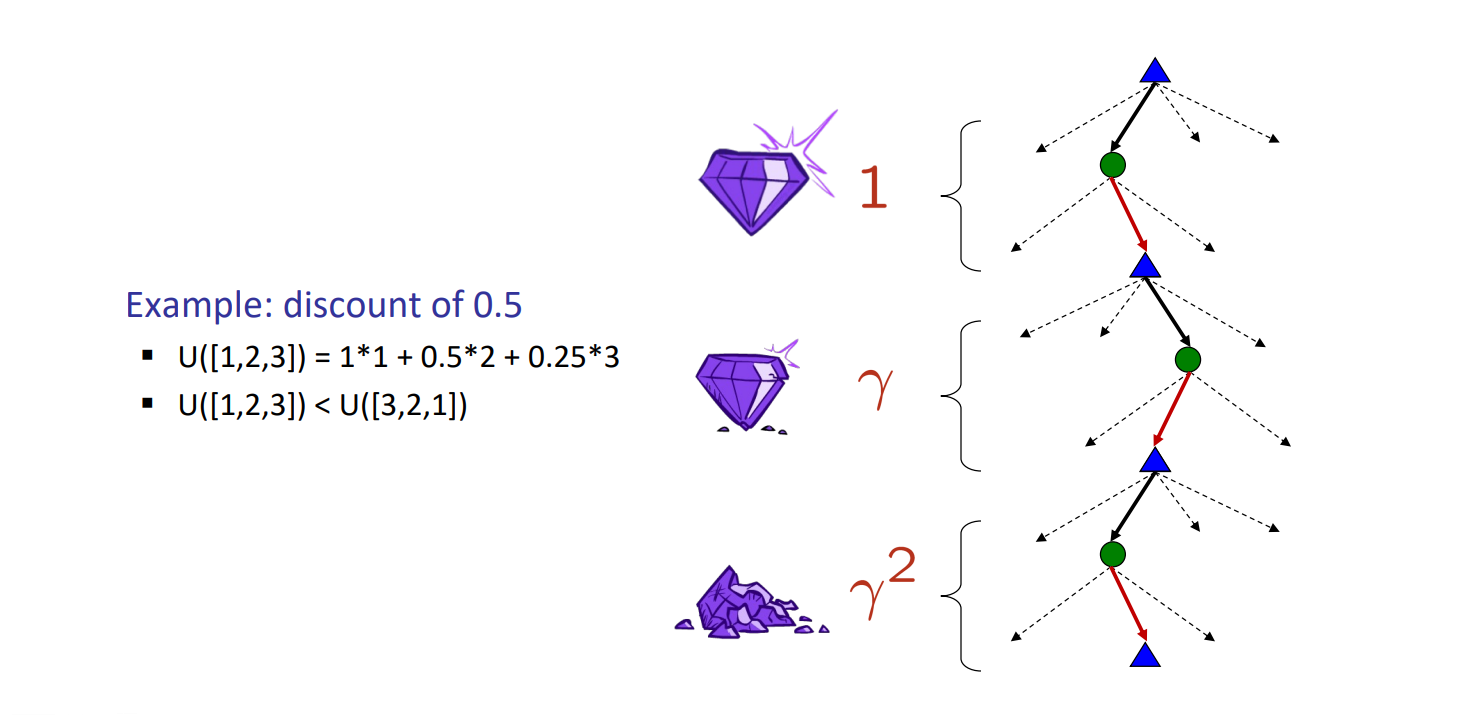
\includegraphics[width=0.7\textwidth]{pictures/discountfac.png}
    \caption{Illustration du discount factor. $U()$ = l'utilité = $Reward \times \gamma^k$}\label{fig:discountfac}
\end{figure}

L'utilité d'une politique $\pi$ est définie comme suit: 
\begin{equation}
    U^\pi(s) = \mathbb{E} \left[ \sum_{k=0}^{\infty} \gamma^k R(s_k, a_k, s_{k+1}) \right] 
\end{equation} 
C'est-à-dire que l'utilité d'une politique est la somme des récompenses futures pondérées par le discount factor.
% \begin{definition}{Utilité}{utility}
%     L'\textbf{utilité} d'un état $s$ est la somme des récompenses futures pondérées par le discount factor: 
%     \begin{equation}
%         U(s) = \sum_{k=0}^{\infty} \gamma^k R(s_k)
%     \end{equation}
%     où $s_k$ est l'état à l'étape $k$. 
% \end{definition}

% subsection Hyper-Parametres (end)

\subsection{Equation de Bellman} % (fold)
\label{sub:equation_de_bellman}

\subsubsection{Quantité optimale} % (fold)
\label{sec:quantite_optimale}

\begin{definition}{Utilité d'un état}{}
    Nous définissions l'utilité d'un état $s$ comme la valeur $V*(s)$. 
    C'est l'utilité espérée à partir de $s$ en suivant la politique optimale $\pi^*$.
    \begin{equation*}
        V^*(s) = \max_{a} Q^*(s, a) 
    \end{equation*}
\end{definition}

\begin{definition}{Utilité d'un q-état}{}
    Nous définissions l'utilité d'un q-état $s, a$ comme la valeur $Q*(s, a)$. 
    C'est l'utilité espérée à partir de $s$ en suivant la politique optimale $\pi^*$ et en effectuant l'action $a$. 
    \begin{equation*}
        Q^*(s, a) = \sum_{s'} T(s, a, s') \left[ R(s, a, s') + \gamma V^*(s') \right]
    \end{equation*}
\end{definition}

\begin{figure}[H]
    \centering
    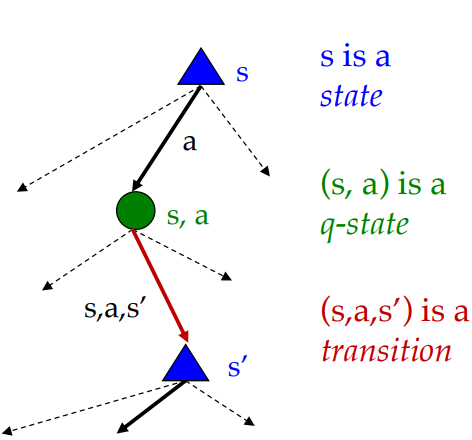
\includegraphics[width=0.3\textwidth]{pictures/bellmantree.png}
    \caption{}\label{fig:}
\end{figure}

\subsubsection{Value Iteration} % (fold)
\label{sec:value_iteration}

\begin{algorithm}[H]
    \caption{Value Iteration}\label{alg:valueiteration}
    \begin{algorithmic}[1]
        \Procedure{ValueIteration}{$S, A, T, R, \gamma, \epsilon$}
            \State $V(s) \gets 0$ for all $s \in S$
            \Repeat
                \State $V_k \gets V$ # Copie de $V$
                \ForAll{$s \in S$}
                    \State $V_k(s) \gets \max_{a} \sum_{s'} T(s, a, s') \left[ R(s, a, s') + \gamma V(s') \right]$
                    % \State $V_(s) \gets \max_{a} \sum_{s'} T(s, a, s') \left[ R(s, a, s') + \gamma V(s') \right]$
                \EndFor
                \State $V \gets V_k$ # Mise à jour de $V$
            \Until{$\max_{s \in S} |V(s) - V'(s)| < \epsilon$}
            \State \textbf{return} $V$
        \EndProcedure
    \end{algorithmic} 
\end{algorithm}

L'algorithme est répété jusqu'à ce que la différence entre $V$ et $V'$ soit inférieure à $\epsilon$. Soit 
ce que l'on appelle la \textbf{convergence}. L'algorithme va converger au bout d'un certain nombre d'itérations.
En effet, plus le nombre d'itérations augmente, plus la différence entre $V$ et $V'$ diminue de part le discount factor $\gamma$ qui devient 
de plus en plus petit.

\textbf{Complexité:} $O(|S|^2 \times |A|)$ 

% subsubsection Value Iteration (end)

\subsubsection{Policy Extraction} % (fold)
\label{sec:policy_extraction}

\begin{algorithm}[H]
    \caption{Policy Extraction}\label{alg:policyextraction}
    \begin{algorithmic}[1]
        \Procedure{PolicyExtraction}{$S, A, T, R, \gamma, V$}
            \State $\pi(s) \gets \argmax_{a} \sum_{s'} T(s, a, s') \left[ R(s, a, s') + \gamma V(s') \right]$
            \State \textbf{return} $\pi$
        \EndProcedure
    \end{algorithmic} 
\end{algorithm}

Cet algorithme permet d'extraire la politique optimale $\pi^*$ à partir de $V^*$. 
En effet, nous pouvons voir que la politique optimale est la politique qui maximise l'utilité. 
Nous pouvons donc extraire la politique optimale à partir de $V^*$ en choisissant l'action qui maximise l'utilité pour chaque état.

% subsubsection Policy Extraction (end)

\subsubsection{Policy Evaluation} % (fold)
\label{sec:policy_evaluation}

Cet algorithme permet de calculer l'utilité d'une politique $\pi$ donnée. 
Il va calculer l'utilité de chaque état en fonction de la politique $\pi$ et de la fonction de transition $T$. 
Il y a moins de calculs à faire que pour l'algorithme de \textbf{Value Iteration} car nous n'avons pas besoin de calculer toutes les valeurs de $V$ à chaque itération. 
Nous avons juste besoin l'utilité d'un état en fonction \textbf{d'une seule} action.

\begin{algorithm}[H]
    \caption{Policy Evaluation}\label{alg:policyevaluation}
    \begin{algorithmic}[1]
        \Procedure{PolicyEvaluation}{$S, A, T, R, \gamma, \pi$}
            \State $V(s) \gets 0$ for all $s \in S$
            \Repeat
                \State $V_k \gets V$ # Copie de $V$
                \ForAll{$s \in S$}
                    \State $V_k(s) \gets \sum_{s'} T(s, \pi(s), s') \left[ R(s, \pi(s), s') + \gamma V(s') \right]$
                \EndFor
                \State $V \gets V_k$ # Mise à jour de $V$
            \Until{$\max_{s \in S} |V(s) - V'(s)| < \epsilon$}
            \State \textbf{return} $V$
        \EndProcedure
    \end{algorithmic} 
\end{algorithm}

Nous pouvons voir que l'algorithme est similaire à l'algorithme de \textbf{Value Iteration} mais que nous n'avons pas besoin de calculer 
la somme des utilités de toutes les actions possibles. Nous avons juste besoin de calculer l'utilité d'une seule action. 
Cela permet de réduire le nombre de calculs à faire.

\textbf{Complexité:} $O(|S|^2)$

\subsubsection{Policy Iteration} % (fold)
\label{sec:policy_iteration}

L'algorithme de \textbf{Policy Iteration} est un algorithme qui permet de trouver la politique optimale $\pi^*$ à partir d'une politique initiale $\pi_0$. 
Il va alterner entre les étapes de \textbf{Policy Evaluation} et \textbf{Policy Extraction} jusqu'à ce que la politique ne change plus. 
La différence avec l'algorithme de \textbf{Value Iteration} est que on commence avec une politique initiale $\pi_0$ et on va la modifier jusqu'à ce qu'elle soit optimale. 
On a donc moins de calculs à faire car on ne va pas devoir calculer toutes les valeurs de $V$ à chaque itération. 

\begin{algorithm}[H]
    \caption{Policy Iteration}\label{alg:policyiteration}
    \begin{algorithmic}[1]
        \Procedure{PolicyIteration}{$S, A, T, R, \gamma, \epsilon$}
            \State $\pi(s) \gets$ random policy
            \Repeat
            \State $V_\pi_{k+1} \gets$ \Call{PolicyEvaluation}{$S, A, T, R, \gamma, \pi$}
            \State $\pi_{i+1} \gets$ \Call{PolicyExtraction}{$S, A, T, R, \gamma, V$}
            \Until{$\pi$ does not change}
            \State \textbf{return} $\pi$
        \EndProcedure
    \end{algorithmic} 
\end{algorithm}

\textbf{Complexité:} $O(|S|^2 \times |A|) + O(|S|^3)$

Cette algorithme est plus lent mais converge plus rapidement que l'algorithme de \textbf{Value Iteration} \textit{(moins d'itérations)}.

\begin{remark}\leavevmode
    Voir exemple slide 22 cours 15.
\end{remark}


% subsubsection Policy Iteration (end)






% subsubsection Quantite optimale (end)


% subsection Equation de Bellman (end)


